\section{Results}

\textbf{Strengths.} The full \texttt{pytest} run passed (247 tests). Most tests are unit-level, which helps catch subtle bugs in logic and resilience math; the smaller set of integration tests targets module boundaries where wiring errors usually appear.

\textbf{Weaknesses.} README filenames still diverge from the tree in places. Tests use hand-built fixtures, not external datasets. We did not run large hyperparameter sweeps or formal UI user studies.

Table~\ref{tab:pytest} lists collection counts by area; every listed test passed in the aggregate run reported above.

\begin{table}[t]
  \centering
  \caption{Tests collected by area (snapshot, April 2026). All passed in the reported full-suite run.}
  \label{tab:pytest}
  \begin{tabular}{@{}lr@{}}
    \toprule
    Area & Tests collected \\
    \midrule
    \texttt{unit\_tests/} & 239 \\
    \texttt{integration\_tests/module2/} & 2 \\
    \texttt{integration\_tests/module3/} & 1 \\
    \texttt{integration\_tests/module4/} & 1 \\
    \texttt{integration\_tests/module5/} & 2 \\
    \texttt{integration\_tests/rl/} & 2 \\
    \midrule
    Total & 247 \\
    \bottomrule
  \end{tabular}
\end{table}

Figure~\ref{fig:qlheat} shows the project's pairwise Q-learning heatmap (copied from \texttt{graphics/ql\_pairwise\_heatmap.png} into \texttt{paper/figures/} for a self-contained paper folder). It is evidence that the learning tooling produces a readable graphic, not a claim about optimal human play; axis and color meaning come from the script that generated the original asset.

If your local clone shows a different total after pulling new commits, update Table~\ref{tab:pytest} and the sentence above to match; do not keep stale counts in the PDF.

Reading Table~\ref{tab:pytest} together with the passing full-suite run supports two narrow claims: first, the low-level pieces (KB, engine, Nash helpers, repeated analysis, RL smoke) each have direct tests; second, a small but targeted set of integration tests guards the interfaces where regressions hurt most. It does \emph{not} support a claim that every feature in the Streamlit UI is exhaustively clicked in CI---only that the underlying Python contracts those screens rely on are exercised.

\begin{figure}[t]
  \centering
  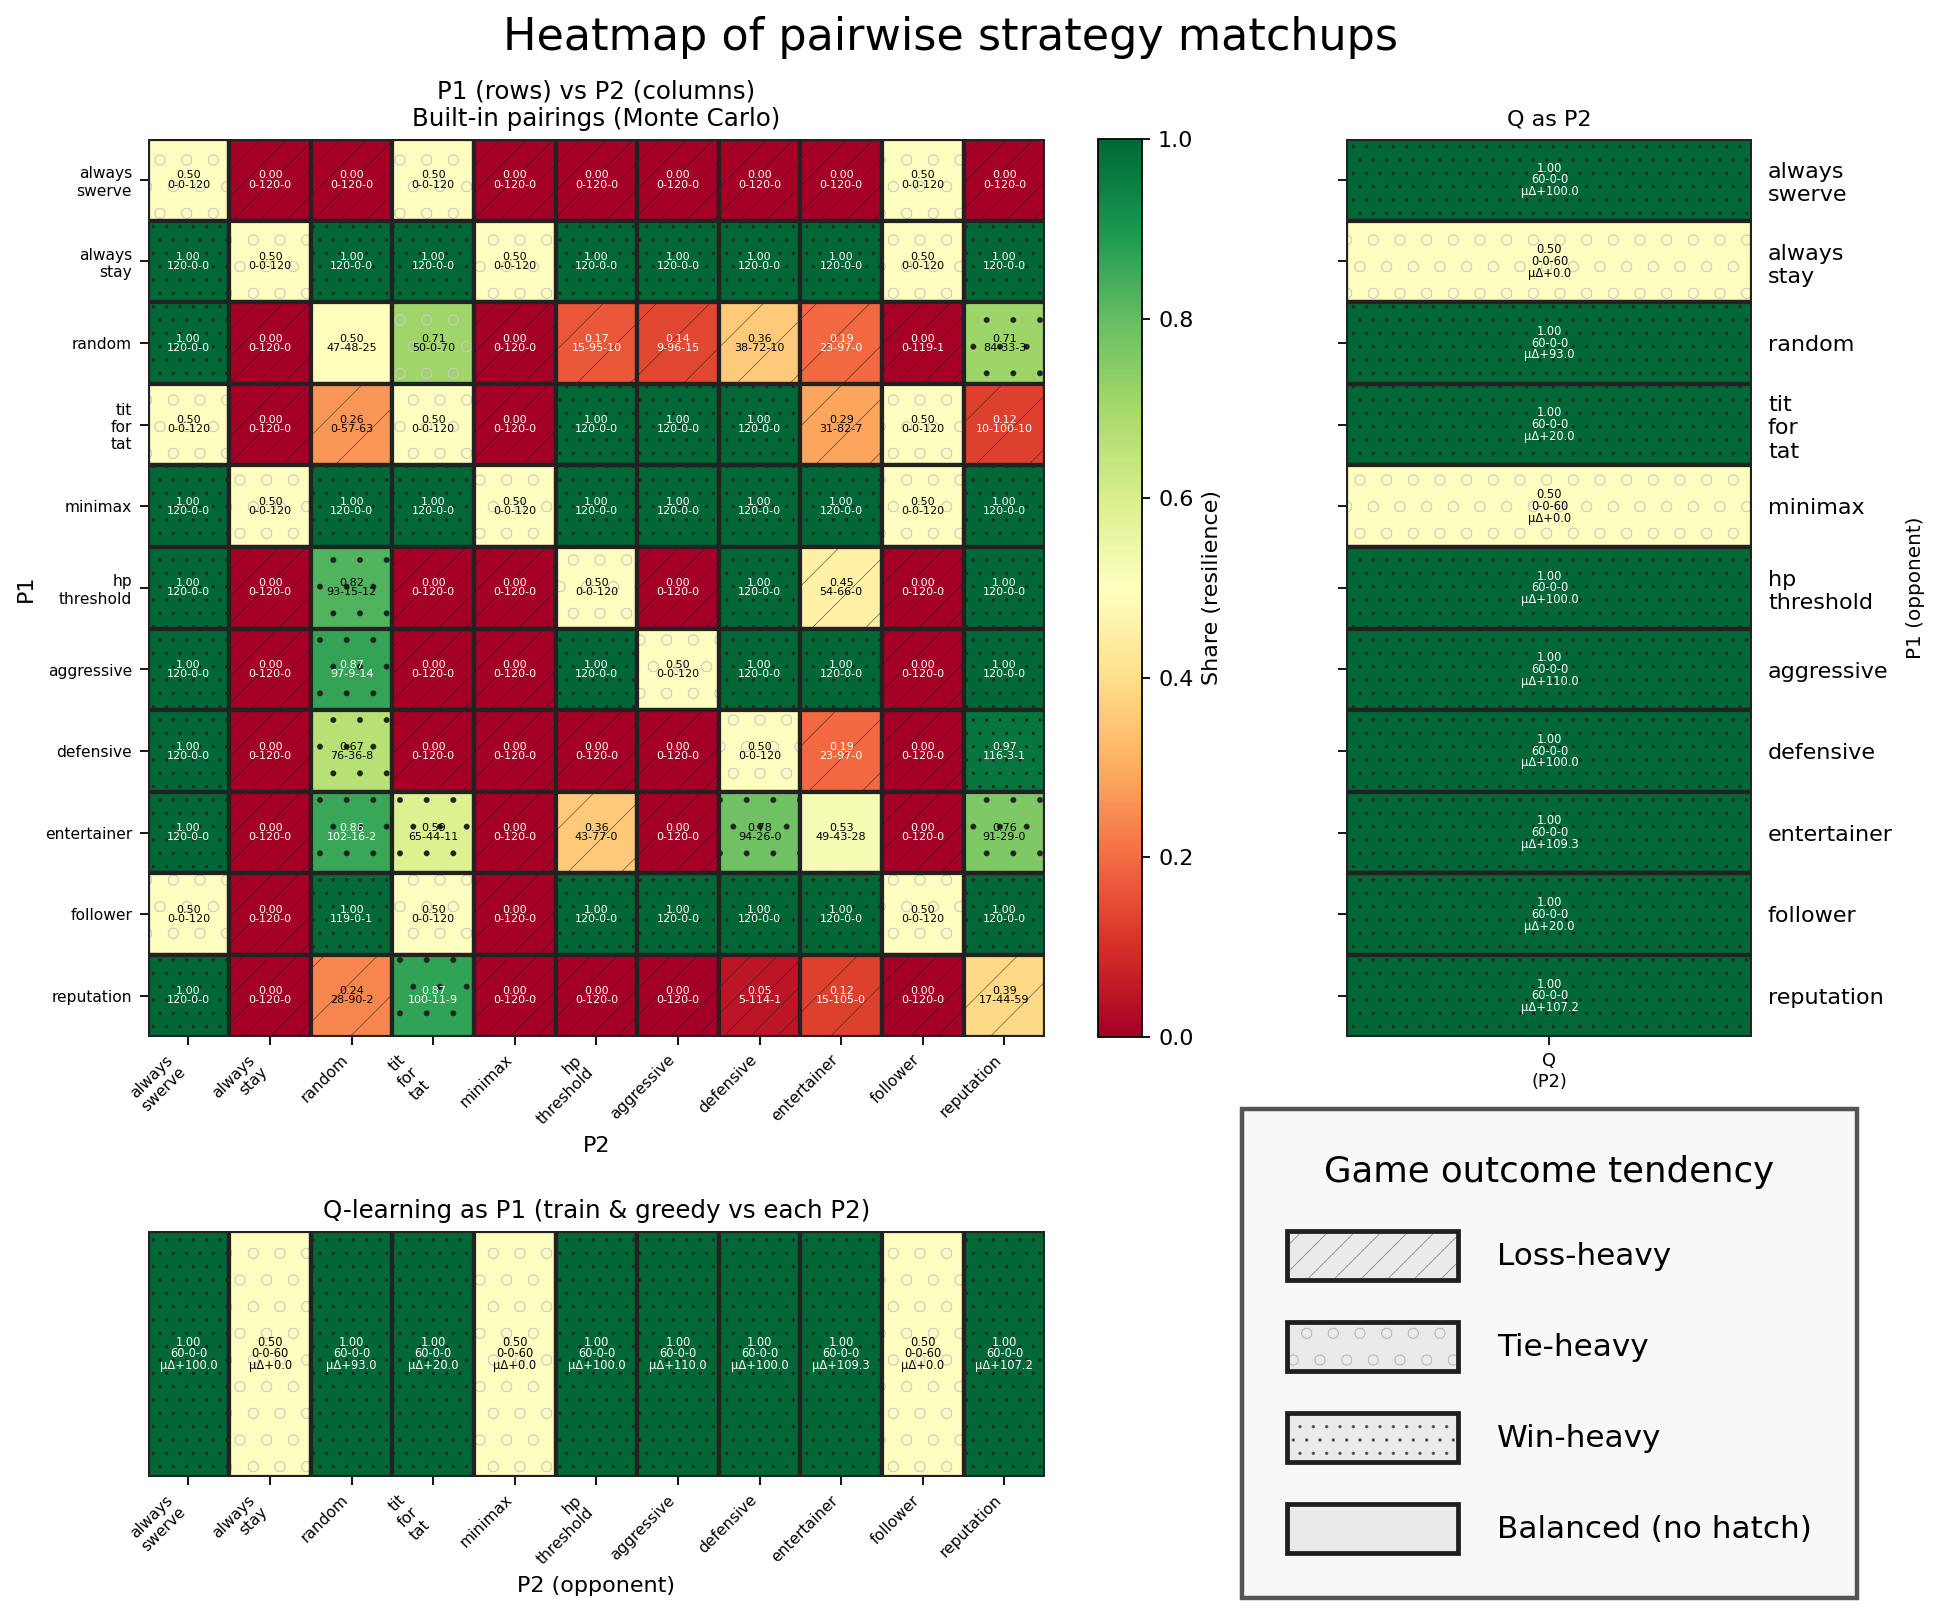
\includegraphics[width=0.72\linewidth]{figures/ql_pairwise_heatmap.png}
  \caption{Pairwise Q-learning heatmap from the project \texttt{graphics/} bundle. Read axis labels and the generator script before citing numeric cells.}
  \label{fig:qlheat}
\end{figure}
